\documentclass[portuguese]{textolivre}

% metadata
\journalname{Texto Livre}
\thevolume{17}
%\thenumber{1} % old template
\theyear{2024}
\receiveddate{\DTMdisplaydate{2023}{12}{8}{-1}}
\accepteddate{\DTMdisplaydate{2024}{3}{12}{-1}}
\publisheddate{\today}
\corrauthor{Cacilda Chivai}
\articledoi{10.1590/1983-3652.2024.49117}
%\articleid{NNNN} % if the article ID is not the last 5 numbers of its DOI, provide it using \articleid{} commmand 
% list of available sesscions in the journal: articles, dossier, reports, essays, reviews, interviews, editorial
\articlesessionname{articles}
\runningauthor{Chivai, Soares \text{and} Catarino}
%\editorname{Leonardo Araújo} % old template
\sectioneditorname{Fernando da Costa Barbosa}
\layouteditorname{João Mesquita}

\title{Qubism 3D Modeling e GeoGebra: softwares adequados para promover a
	visualização 3D nos temas de projeção ortogonal e seção de cilindros}
\othertitle{Qubism 3D Modeling and Geogebra: Suitable Softwares to Promote 3D
	Visualization in the Topics of Ortogonal Projections and Cylinder
	Sections}

\author[1]{Cacilda Helena Chivai~\orcid{0000-0003-4365-4891}\thanks{Email: \href{mailto:cacildachivai@gmail.com}{cacildachivai@gmail.com}}}
\author[2,4]{Armando Assunção Soares~\orcid{0000-0003-1860-2432}\thanks{Email: \href{mailto:asoares@utad.pt}{asoares@utad.pt}}}
\author[3,5]{Paula Catarino~\orcid{0000-0001-6917-5093}\thanks{Email: \href{mailto:pcatarin@utad.pt}{pcatarin@utad.pt}}}
\affil[1]{Universidade Pedagógica de Maputo, Faculdade de Engenharias e Tecnologias, Departamento de Desenho, Maputo, Moçambique.}
\affil[2]{Universidade de Trás-os-Montes e Alto Douro, Escola de Ciências e Tecnologia, Departamento de Física, Vila Real, Portugal.}
\affil[3]{Universidade de Trás-os-Montes e Alto Douro, Escola de Ciências e Tecnologia, Departamento de Matemática, Vila Real, Portugal.}
\affil[4]{INEGI/LAETA Instituto de Ciência e Inovação em Engenharia Mecânica e Engenharia Industrial, Portugal.}
\affil[5]{CIDTFF - Centro de investigação da Universidade de Aveiro.}

\addbibresource{article.bib}

\begin{document}
\maketitle
\begin{polyabstract}
\begin{abstract}
No Ensino Secundário Geral em Moçambique, ainda é raro o uso de
recursos tecnológicos para o aprendizado de Desenho Técnico e de
Geometria Descritiva. O objetivo desta pesquisa é verificar se as
simulações dos \textit{softwares} Qubism 3D Modeling e GeoGebra, nos temas de
Projeção Ortogonal e de Seção de Cilindros, contribuem para a formação
de alunos nesse tipo de habilidade. Para o estudo das Projeções
Ortogonais, adaptamos o Qubism 3D Modeling para ajudar na clarificação
das representações das vistas ortogonais. Para o estudo das seções
produzidas em cilindro, utilizamos o \textit{software} de geometria dinâmica
GeoGebra, por facilitar a percepção da forma da figura resultante da
seção. Este estudo é quase-experimental, seguindo uma abordagem
qualitativa, conduzido em uma escola do sul de Moçambique. As técnicas
empregadas incluíram observação, tomadas de notas e registros
fotográficos, e os instrumentos utilizados foram questionários de
satisfação. Participaram 50 alunos, dos quais 25 experimentaram o
\textit{software} Qubism 3D Modeling e os 25 restantes utilizaram o \textit{software}
GeoGebra. Esses alunos resolveram exercícios práticos de Desenho Técnico
e de Geometria Descritiva durante a intervenção didática. A análise dos
resultados sugere que os alunos desenvolveram competências de
visualização espacial, e os dados também indicaram que os \textit{softwares}
aplicados promoveram aprendizagens significativas, possibilitando
verificar o aprendizado resultante das simulações computacionais. A
partir da pesquisa já realizada, existem algumas curiosidades e
percepções que podem servir de ponte para novas pesquisas sobre a
aplicabilidade da tecnologia no estudo de diversos temas de Desenho
Técnico e de Geometria Descritiva.

\keywords{Simulações computacionais \sep Qubism 3D Modeling \sep
	Software de geometria dinâmica Geogebra \sep Projeções ortogonais \sep Seções de cilindros.}
\end{abstract}

\begin{english}
\begin{abstract}
In General Secondary Education in Mozambique, the use of
technological resources for learning Technical Drawing and Descriptive
Geometry is still rare. The aim of this research is to see if Qubism 3D
Modeling and GeoGebra software simulations, in the subjects of
Orthogonal Projection and Section of Cylinders, contribute to improving
students 3D spatial visualization, considering students previous difficulties in this type of skill. For the study of Orthogonal Projections, we adapted Qubism 3D Modeling to help clarify the representations of orthogonal views. For the study of cylinder sections, we used the dynamic geometry software GeoGebra, as it facilitates the perception of the shape of the figure resulting from the section. This is a quasi-experimental study, following a qualitative approach, conducted in a school in southern Mozambique. The techniques employed included observation, note-taking and photographic records, and the instruments used were satisfaction questionnaires. Fifty students took part, 25 of whom tried out the Qubism 3D Modeling software and the rest used the GeoGebra software. These students solved practical
exercises in Technical Drawing and Descriptive Geometry during the
didactic intervention. The analysis of the results suggests that the
students developed spatial visualization skills, and the data also
indicates that the software applied promoted significant learning,
making it possible to verify the learning resulting from the computer
simulations. From the research already carried out, there are some
curiosities and perceptions that can serve as a bridge for further
research into the applicability of technology in the study of various
subjects in Technical Drawing and Descriptive Geometry.

\keywords{Computer simulations \sep Qubism 3d modeling \sep GeoGebra
	dynamic geometry software \sep Orthogonal  projections \sep Cylinder sections}
\end{abstract}
\end{english}
\end{polyabstract}

\section{Introdução}\label{sec-intro}

O processo de escrita é uma das atividades mais complexas que o ser
humano é capaz de realizar, em razão de vários fatores, a exemplo das
exigências feitas à memória e ao raciocínio durante o momento de
produção \cite{garcez2020}. São inúmeros os conhecimentos e habilidades que
precisam ser articulados e harmonizados para que o texto tome forma.
Tendo em vista esse seu caráter complexo, ainda são recorrentes falsas
crenças sobre a produção textual, que levam pessoas a acreditarem que
podem dominá-la a partir de ``dicas'' desvinculadas de seu contexto de
produção.

A ideia de que fórmulas pré-fabricadas e ``dicas'' isoladas são métodos
cabíveis no ensino de produção textual, apenas negligencia as etapas
necessárias que caracterizam um texto adequado conforme seu contexto de
produção \cite{garcez2020}. O processo de escrita é uma atividade que
carece de idas e vindas, pois deve admitir três grandes momentos que se
intercalam e devem ser compreendidos de modo indissociável: o do
planejamento, o da escrita propriamente dita e o da revisão \cite{antunes2005}. Enquadrar esse processo em uma perspectiva prescrita e linear
pode resultar em estudantes frustrados pela construção de textos
truncados e artificiais.

Essa realidade se agrava quando observamos o cenário acadêmico, em que
as exigências com relação a produções textuais se intensificam. As
expectativas quanto a essas produções não se limitam à utilização
adequada da norma-padrão ou a vocabulários específicos; expandem-se para
aspectos implícitos de produção que precisam ser considerados, como o
que pode ser dito, por quem, de que forma, sob que ponto de vista e
fundamentado em qual autor \cite{oliveira2024}.

Pensando na comunidade discursiva acadêmica, uma das produções textuais
mais demandadas em cursos de graduação da área de humanas é o artigo
acadêmico \cite{motta-roth2010}. Por ser um dos principais
veículos de divulgação científica, a circulação desse gênero na academia
é incontornável, sendo bastante exigido o seu consumo e produção por
parte de professores, estudantes e pesquisadores. Embora seja uma
produção essencialmente ligada ao meio universitário, sua feitura é
quase sempre exigida sem antes ser ensinada. Esse fato pode levar os
alunos a somarem suas dificuldades com o processo de escrita à
dificuldade de produzir um texto do qual desconhecem seu contexto de
produção, estrutura composicional e outras ``dimensões escondidas''
\cite{street2010} que perpassam a construção de um artigo.

Ao exigir do autor capacidade de síntese, descrição, análise e
argumentação, utilizando-se das convenções próprias à determinada área,
o artigo contempla informações geradas em pesquisas a serem submetidas a
apreciações públicas \cite{motta-roth2010}. Sua relevância remonta
à popularização da ciência que, por sua vez, possui a potencialidade de
descrever fenômenos sociais e até mesmo gerar algum impacto benéfico ao
público em geral.

A partir dessas pontuações, torna-se clara a importância de produzir
artigos acadêmicos e a responsabilidade do seu produtor de popularizar
os conhecimentos produzidos na esfera acadêmica. Quando essa tarefa de
produção precisa ser desenvolvida por graduandos e estes normalmente não
recebem orientação para tal, muitas vezes, recorrem a materiais digitais
sobre esse assunto, pois lhes propiciam as mais variadas estratégias de
ensino de acordo com o ritmo e as preferências do estudante \cite{falkembach2005}. Um fator que pode justificar essa recorrência é a facilidade de
acesso a plataformas digitais, que disponibilizam, na maioria das vezes
de forma gratuita, conteúdos digitais educacionais. Antigamente, os
estudantes consultavam manuais impressos que ensinavam a como produzir
textos acadêmicos, hoje, frente aos recursos tecnológicos, os locais de
aprendizagem se ampliam para a cibercultura. Como cibercultura,
compreendem-se vários ambientes da esfera digital que abrigam
informações, até mesmo os que simulam uma sala de aula a partir de
vídeos \cite{martins2018,rocha2005}.

Tendo a cibercultura se tornado uma potencializadora de novas abordagens
educativas, deve-se averiguar sua eficiência enquanto ferramenta de
ensino, a forma como se ensina determinados conteúdos, a exemplo da
produção textual de artigo acadêmico e seus aspectos constitutivos, foco
do presente estudo. Nesse sentido, traçamos dois objetivos para este
trabalho: identificar e analisar objetos de ensino explorados em
videoaulas sobre artigo acadêmico publicadas na plataforma YouTube.

Para tanto, organizamos este artigo em 5 seções, a saber: esta
introdução, contendo uma contextualização inicial sobre o objeto de
investigação da pesquisa, a problemática que o envolve e os objetivos
delineados; o embasamento teórico, no qual apresentamos os pressupostos
que fundamentam o estudo --- as práticas de ensino de Língua Portuguesa
em contexto didático-digital \cite{laurentino2023}, o artigo
acadêmico \cite{motta-roth2010}, as etapas de produção textual
(Antunes, 2003) e os objetos de ensino \cite{linodearaujo2014}; a
metodologia, na qual explicitamos a abordagem e o tipo de pesquisa, bem
como os procedimentos de coleta e análise de dados; os resultados,
contendo a exploração dos objetos de ensino contemplados nas videoaulas
sobre ensino de produção de artigo acadêmico; as considerações finais,
nas quais sinalizamos algumas implicações advindas dos resultados
alcançados.
% !TeX root = main.tex

\section{Metodología}\label{sec-metodología}

La metodología de la investigación la entendemos como el conjunto de
procedimientos y técnicas que el equipo investigador ha utilizado en el
diseño, desarrollo y análisis del estudio. En este caso concreto, el
método utilizado ha sido de corte mixto, utilizando técnicas
cualitativas y cuantitativas. Las cualitativas se han basado en la
etnografía virtual de los datos generados en los sNOOC y las
conclusiones del juicio del equipo de expertos. Las cuantitativas
provienen de los cuestionarios de satisfacción del alumnado y de los
datos de interacción del alumnado en la plataforma de aprendizaje.


\subsection{Objetivos e hipótesis}\label{sub-sec-objetivosehipotesis}

El objetivo general de este estudio es analizar el proceso de creación
de redes comunicativas de estudiantes para la implementación de sNOOC
como método de evaluación continua en la UAD y su repercusión en la capa
social como modelo de formación mediática en personas de la tercera
edad. Con base en este objetivo general, los objetivos específicos hacen
referencia a:

\begin{itemize}
\item
Objetivo Específico 1 (OE1): Investigar las percepciones y opiniones
de las redes comunicativas de estudiantes respecto a la utilidad y
efectividad de un sNOOC como método de evaluación continua y su
impacto en la motivación hacia el aprendizaje.
\item
Objetivo Específico 2 (OE2): Examinar el proceso de desarrollo de las
redes comunicativas de estudiantes para la creación de contenidos de
los sNOOC, centrándose en el impacto del uso de pedagogías inclusivas,
IA y Metaverso en EAD.
\item
Objetivo Específico 3 (OE3): Evaluar el nivel de implicación activa de
las redes comunicativas de estudiantes en la plataforma de la UNED y
en la creación colaborativa del sNOOC en tmooc.es.
\end{itemize}

A continuación, se formulan las hipótesis para dar respuesta a las
relaciones causales:

\begin{itemize}
\item
Hipótesis 1 (H1-OE1): Si las redes comunicativas de estudiantes
perciben el sNOOC como una herramienta efectiva y útil para la
evaluación continua, aumentará su motivación intrínseca hacia el
aprendizaje y su participación en las actividades y recursos del
itinerario de aprendizaje propuesto.
\item
Hipótesis 2 (H2-0E2): Si el modelo sNOOC es diseñado y aplicado
considerando criterios pedagógicos inclusivos y herramientas
tecnológicas adecuadas, mejorará la comprensión de los contenidos por
parte de las redes comunicativas de estudiantes, incrementando su
satisfacción general con la experiencia de EAD.
\item
Hipótesis 3 (H3-OE3): Si el itinerario de aprendizaje en sNOOC está
basado en pedagogías inclusivas, se incrementará el compromiso activo
de las personas participantes, reflejado en una mayor interacción,
colaboración en equipo y corresponsabilidad en la construcción
colectiva del conocimiento.
\end{itemize}


\subsection{Muestra, instrumentos y análisis de
	datos}\label{sub-sec-muestrainstrumentos}
	
	El objeto de estudio de esta investigación son las interacciones del
	alumnado en la plataforma ALF de la UNED, contando con la participación
	de 79 personas, 57 mujeres y 22 hombres; 1 de nacionalidad croata y, el
	resto, española. Estos participantes han sido estudiantes del Máster
	Universitario en Educación y Comunicación en la Red y, dentro de este,
	de la asignatura ``Escenarios Virtuales para la participación'', una
	disciplina con contenidos relacionados con la educación mediática. En
	este caso concreto, para estructurar el método cuantitativo, se han
	utilizado los cuestionarios con preguntas diseñadas para recopilar datos
	cuantitativos correspondiente al curso 2023/2024.
	
	Referido a la plataforma ``tmooc.es'' donde este grupo de estudiantes
	creó los sNOOC, se ha realizado un análisis de estas propuestas tomando
	también esos entornos como objeto de estudio. Se tuvieron en cuenta los
	registros de datos relacionados con la dedicación en la creación de los
	sNOOC. Los sNOOC seleccionados son los siguientes: ``Introdúcete al
	mundo de Facebook'' (sN1), ``Senior 3.0'' (sN2), ``Correo electrónico
	son misterios: alfabetización digital para personas mayores'' (sN3),
	``Enredados en la edad dorada: dominar Facebook e Instagram con
	confianza'' (sN4), ``Healthy seniors network'' (sN5), ``Estas a un clic
	de conocer el mundo digital'' (sN6), ``Familias y aprendizaje en red''
	(sN7) y ``Google e inteligencia artificial, tus compañeros digitales''
	(sN8). En cuanto al enfoque cualitativo, se consideraron los datos
	generados a través de los sNOOC y las conclusiones del juicio de 22
	personas expertas internacionales, con el fin de validar hipótesis y
	evaluar riesgos o problemáticas presentes en el proyecto formativo. Para
	analizar los datos cuantitativos y cualitativos se utilizaron los
	programas SPSS y Atlas.ti, respectivamente. Estos aspectos se han
	organizado en categorías que se ajustan a las dimensiones de la
	educación inclusiva.

% !TeX root = main.tex


\section{Resultados}\label{sec-resultados}
Los resultados de este estudio se han organizado en torno a dos
categorías fundamentales. En primer lugar, la Categoría 1 hace
referencia a ``Acceso, equidad y participación''; y, en segundo lugar,
la Categoría 2, se refiere a ``Respecto a la diversidad, colaboración y
prácticas pedagógicas inclusivas''. Estas dimensiones son
interdependientes y mantienen sinergias con el fin de promover la
equidad, la diversidad, la participación y el éxito del proyecto de
alfabetización mediática para personas de la tercera edad.
	

\subsection{Categoría 1: Acceso, equidad y participación}\label{sub-sec-categoría}
	

\subsubsection{Subcategoría: Acceso a la plataforma digital}\label{sub-sub-sec-subcategoríaacessoala}
	
El acceso a la plataforma de la asignatura ``Escenarios Virtuales para
la Participación'' desde donde se ha proyectado la red comunicativa nos
da a conocer, a nivel de tiempo y dedicación, la actuación como
interactuados de las y los estudiantes, tanto en términos de frecuencia
como de tiempo dedicado. El análisis de los datos de acceso y
participación revela diversos patrones: determinados estudiantes
muestran registros de acceso mínimos, en contraste, otras y otros
estudiantes con niveles de acceso significativamente altos, con datos
que acceden a 3436 y 1981 respectivamente. La cantidad de sesiones varía
también significativamente, con estudiantes que participan en 736 y 123
sesiones respectivamente, lo cual, indica un rol de interactuado
frecuente y prolongado en la plataforma. En este sentido, el acceso nos
remite a la posible participación, otro aspecto de esta categoría,
reflejando diversidad de hábitos de estudio y nivel de compromiso del
alumnado.
	
Los datos recopilados se han analizado en tres métricas que hacen
referencia a accesos, minutos y sesiones. El valor medio sugiere que, en
promedio, se han efectuado 520 accesos, utilizando 2575 minutos y
desarrollándose unas 41680 sesiones. La mediana, representando el valor
central de los datos ordenados, muestra que la mitad de los valores se
sitúan encima y la otra mitad por debajo de 3755 accesos, 20 minutos y
25 sesiones. El valor modal, es decir, aquel que aparece con mayor
frecuencia, señala que el número más común de accesos es 2, mientras que
los valores predominantes para el tiempo y el número son 0 minutos y 1
sesión. El total acumulado de accesos, minutos y sesiones es 43695, 2163
y 3501. Los valores mínimos y máximos ilustran el rango de los datos,
con un mínimo de 1 acceso y un máximo de 3436.
	
En términos de tiempo, el mínimo registrado es 0 minutos, indicando
periodos de inactividad, mientras que el máximo es 96 minutos.
Concretamente, para el tiempo dedicado a las sesiones, el rango es
variable, entre 1 y 736. Estos datos, representados en la \Cref{fig-01},
ofrecen una comprensión detallada de la actividad de acceso, el tiempo
dedicado y el número de sesiones, esencial para analizar las
interacciones y los patrones de comportamiento del alumnado en la
plataforma. Con base en los datos sobre el tiempo de permanencia en la
plataforma, según la \Cref{fig-02}, se observa una distribución heterogénea
en las horas dedicadas al estudio por parte de las personas que forman
la red comunicativa. Un 38,9~\% dedica entre 2 y 4 horas de estudio; un
27,8~\% entre 2 y 4 horas; un 16,7\% de las personas participantes entre
6 y 8 horas; y un 11,1~\% reporta estudiar más de 8 horas.
	
\begin{figure}[htbp]
\centering
\begin{minipage}{.85\textwidth}
\caption{Tiempo accesos minutos.}
\label{fig-01}
\includegraphics[width=\textwidth]{Imagem1.png}
\source{Elaboración propia.}
\end{minipage}
\end{figure}
	
\begin{figure}[htbp]
\centering
\begin{minipage}{.85\textwidth}
\caption{Tiempo de estudio.}
\label{fig-02}
\includegraphics[width=\textwidth]{Imagem2.png}
\source{Elaboración propia.}
\end{minipage}
\end{figure}		

Al referirnos a la valoración global de la asignatura, nos proporciona
una información valiosa sobre aspectos de la equidad en el contexto
educativo. Según se presenta en la \Cref{fig-03} sobre los tramos de ítem,
los resultados muestran una progresión, destacando una mayor atención a
la adecuación, coherencia y satisfacción global. El tramo 1, la mediana
es 14,4, con un rango intercuartílico (IQR) desde 5,6 hasta 44,4; en el
tramo 2, la mediana es de 15,7, con un IQR desde 5,6 hasta 43,9; en el
tramo 3, la mediana es de 41,0, y el IQR abarca desde 27,8 hasta 55,6;
en el tramo 4, la mediana se encuentra en 33,3, con un IQR desde
aproximadamente 5,6 hasta 55,6. En los tramos 1, 2 y 4 se identifican
valores atípicos en ambos extremos.
	
\begin{figure}[htbp]
	\centering
    \begin{minipage}{.85\textwidth}
	\caption{Valoración de la asignatura.}
	\label{fig-03}
	\includegraphics[width=\textwidth]{Imagem3.png}
	\source{Elaboración propia.}	
    \end{minipage}
\end{figure}
	
\subsubsection{Subcategoría: Equidad en el acceso, desempeño y evaluación}\label{sub-sub-sec-equidadenelacceso}
	
Según se evidencia en la \Cref{fig-04}, tramo 1, el alumnado muestra un mayor
nivel de conocimientos previos (44,4~\%), con adecuación entre la carga
de trabajo y créditos de la asignatura (16,7~\%). En el tramo 2 la
satisfacción global sobre los recursos y apoyo (50~\%) y utilidad del
plan de trabajo para la preparación de la asignatura (27,8~\%) son
aspectos bien valorados. En el tramo 3, resalta la coherencia de los
contenidos con el conjunto del máster (38,9~\%); y la percepción
equitativa sobre los datos contenidos en la guía de estudio (44,4~\%).
En el tramo 4, la satisfacción global con el equipo docente (55,6~\%) y
la atención inclusiva que el mismo presta a los foros (47,1\%) son
aspectos altamente valorados. Se observa una distribución variada en la
valoración de la asignatura en diferentes aspectos y tramos, lo que
sugiere que la percepción de las y los estudiantes puede verse
influenciada por diferentes factores a lo largo del curso.
	
\begin{figure}[htbp]
\centering
\begin{minipage}{.85\textwidth}
\caption{Valoración de asignatura por tramos.}
\label{fig-04}
\includegraphics[width=\textwidth]{Imagem4.png}
\source{Elaboración propia.}	
\end{minipage}
\end{figure}
	
En lo atinente a la valoración de la asignatura en relación con otras,
se puede verificar según presenta la \Cref{fig-05} que esta disciplina recibe
valoraciones bastante altas en todos los ítems evaluados, con puntajes
que oscilan entre 36,15~\% y 81,7~\%, observando una percepción positiva
en cuanto a la interacción que se proyecta. Aspectos como "La coherencia
de los contenidos de la asignatura con el conjunto del máster" y "Los
conocimientos adquiridos en esta asignatura", son más altas, indicando
una fuerte percepción de coherencia y utilidad de los contenidos en
relación con el programa y un alto grado de aprendizaje. Otras
referencias a "La adecuación del material didáctico para el estudio de
esta asignatura" y "La utilidad del curso virtual para la preparación de
la asignatura" muestran puntajes más bajos, indicando que podría haber
margen de mejora sobre la calidad y la utilidad de las herramientas
comunicativas y recursos presentados. Los ítems tienen un margen de
error estimado medio o bajo, lo que sugiere que las estimaciones de las
puntuaciones son bastante precisas y fiables. Esta disciplina está bien
valorada y aumenta su valoración cada año, según presenta la \Cref{fig-06},
con ámbitos específicos que podrían beneficiarse a nivel de inclusión
como las herramientas comunicativas, los recursos y la metodología.
	
\begin{figure}[htbp]
	\centering
    \begin{minipage}{.85\textwidth}
	\caption{Valoración de asignatura en relación con otras.}
	\label{fig-05}
	\includegraphics[width=\textwidth]{Imagem5.png}
    \source{Elaboración propia.}
    \end{minipage}
\end{figure}

\begin{figure}[htbp]
	\centering
    \begin{minipage}{.85\textwidth}
	\caption{Valoración de asignatura por año.}
	\label{fig-06}
	\includegraphics[width=\textwidth]{Imagem6.png}
	\source{Elaboración propia.}
    \end{minipage}
\end{figure}
	
En la \Cref{fig-07} se pone de manifiesto cómo el alumnado distribuye su
tiempo, lo que puede reflejar la accesibilidad a los recursos y el
tiempo de desempeño. Los documentos, las tareas y calificaciones son las
herramientas que requieren más tiempo, con 4190 y 2202 minutos
respectivamente.

\begin{figure}[htbp]
\centering
\begin{minipage}{.85\textwidth}
\caption{Tiempo accesos minutos por recurso.}
\label{fig-07}
\includegraphics[width=\textwidth]{Imagem7.png}
\source{Elaboración propia.}
\end{minipage}
\end{figure}
	

\subsubsection{Subcategoría: Participación y red comunicativa}\label{sub-sub-sectionparticipación}
	
El análisis de los diferentes textos que se presentan en los foros de la
plataforma nos otorga información clave sobre el proceso de creación de
la red que se puede estructurar en torno a cinco puntos:
	
\begin{itemize}
\item
Búsqueda y formación de grupos: personas participantes están buscando
semejantes con intereses similares.
\item
Presentación personal: cada persona ofrece una breve presentación,
destacando su experiencia, formación y motivaciones para unirse al
proyecto de formación mediática. Esto ayuda a crear una red específica
teniendo presente los antecedentes y perspectivas personales.
\item
Diversidad de participantes: las personas provienen de lugares
geográficos distintos, con diferentes áreas de especialización como
enseñanza de idiomas, tecnología educativa, pedagogía, etc. Así, las
discusiones son más enriquecedoras y los proyectos formativos con
variedad de perspectivas.
\item
Intereses comunes: a pesar de la diversidad formativa y de
proveniencia geográfica, tienen como interés común la pedagogía
digital, la tecnología educativa y la innovación en la enseñanza. Esto
consolida la red comunicativa en base a un objetivo concomitante.
\item
Inclusión, colaboración y apoyo mutuo: disposición a colaborar y
apoyarse mutuamente en la formación de grupos, reflejando espíritu
colaborativo y solidario intencional de cara al proyecto formativo que
se quiere desarrollar.
\end{itemize}

A juzgar por estas cuestiones analizadas, se puede comprobar cómo la
conversación desarrollada en el foro manifiesta un ambiente colaborativo
y participativo con un alumnado comprometido con la creación colectiva
del conocimiento y la aplicación práctica de los conceptos aprendidos en
el itinerario de aprendizaje. El uso intensivo de los foros es un
componente esencial en la organización de las redes comunicativas, base
del proyecto de alfabetización mediática.

Con una correlación positiva significativa entre accesos y sesiones ($r =
0.81$, $p < 0.001$), y una correlación moderada entre accesos y
minutos ($r = 0.5$, $p < 0.001$), nos indica que las personas
participantes, además de acceder a los foros con frecuencia, invierten
un tiempo considerable en ellos. Esto favorece la formación de grupos
con intereses similares y permite a cada participante destacar su
experiencia y motivaciones. A pesar de la diversidad de las y los
componentes de las diferentes redes, que provienen de diferentes lugares
y áreas de especialización, los intereses comunes fortalecen la red. La
disposición a colaborar y apoyarse mutuamente se refleja en el uso
intensivo de los foros, fomentando un espíritu de inclusión y
solidaridad en el proyecto formativo. La correlación moderada entre
minutos y sesiones ($r = 0.36$, $p = 0.001$) sugiere que un mayor tiempo en
los foros está asociado con un mayor número de sesiones. Sin embargo, el
número no muestra una relación significativa con accesos ($r = -0.04$, $p =
0.716$), minutos ($r = 0.07$, $p = 0.533$) o sesiones ($r = -0.09$, $p = 0.425$),
lo que indica que el número total de usuarios no afecta
significativamente estos parámetros. Esto subraya la importancia de la
calidad de la interacción sobre la cantidad de personas en el éxito del
proyecto formativo. La alta frecuencia de uso de los foros facilita
también la búsqueda y formación de grupos, donde las personas
participantes buscan intereses similares; refleja un espíritu de
inclusión, colaboración y apoyo mutuo, crucial para la formación de
grupos colaborativos y solidarios en el proyecto formativo, según
observamos en la \Cref{fig-08}.

\begin{figure}[htbp]
\centering
\begin{minipage}{\textwidth}
\caption{Interacción en los foros.}
\label{fig-08}
\includegraphics[width=\textwidth]{Imagem8.png}
\source{Elaboración propia.}
\end{minipage}
\end{figure}

El diagrama de Sankey, presentado en la \Cref{fig-09}, muestra cómo las y los
participantes, a través de su autoconocimiento y desarrollo personal,
buscan a semejantes con intereses similares para formar redes. Esto se
refleja en las conexiones que fluyen desde "Autoconocimiento" y
"Desarrollo personal" hacia otros nodos en el diagrama. En cuanto a la
``Presentación personal'', las y los participantes presentan sus
antecedentes y motivaciones, lo que ayuda a formar una red específica.
Esto se puede ver en las conexiones que fluyen desde "Autoconocimiento"
y "Desarrollo personal" hacia "Interacción" y "Motivación". En lo que
respecta a ``Diversidad de participantes'', aparece reflejada en el nodo
"Diversidad", enriquece las discusiones y los proyectos formativos. Las
conexiones que fluyen desde "Diversidad" hacia otros nodos indican cómo
ésta se integra en el proyecto. Con respecto a ``Intereses comunes'', a
pesar de la diversidad, las y los participantes tienen un interés común
en la pedagogía digital, la tecnología educativa y la innovación. Esto
se refleja en las conexiones que fluyen hacia y desde el nodo
"Educación". En cuanto a inclusión, colaboración y apoyo mutuo: la
disposición se refleja en el uso intensivo de los foros, promoviendo un
espíritu de inclusión y solidaridad en el proyecto formativo. Esto se
puede ver en las conexiones que fluyen hacia y desde el nodo
"Interacción".

\begin{figure}[htbp]
	\centering
    \begin{minipage}{\textwidth}
	\caption{Formación de redes comunicativas y conexiones de participantes.}
	\label{fig-09}
	\includegraphics[width=\textwidth]{Imagem9.png}
	\source{Elaboración propia.}	
    \end{minipage}
\end{figure}


\subsection{Categoría 2: Diversidad, colaboración y prácticas pedagógicas inclusivas}\label{sub-section-diversidad}
	
	
\subsubsection{Subcategoría: Plataforma digital para la diversidad}\label{sub-sub-sec-subcategoríaplataformadigital}
	
La plataforma ``tmooc.es'' donde se ha desarrollado este proyecto es
Chamilo, de código abierto y con múltiples funcionalidades para la
creación de sNOOC. Partiendo de un aspecto clave como es la diversidad,
analizamos si es real en el proyecto formativo y si se está garantizando
que todas las personas, independientemente de sus características o
capacidades, puedan ejercer el derecho a la inclusión y la igualdad de
oportunidades. Referido a la accesibilidad, Chamilo proporciona diversas
herramientas para la creación de contenidos accesibles desde el diseño
universal, incluyendo todo tipo de dificultad: contenido multimedia con
subtítulos, crear contenido estructurado y navegable, personalizar
diseño compatible con lectores de pantalla y otros asistentes
tecnológicos. Además, esta plataforma posibilita también el uso adecuado
de etiquetas semánticas HTML y descriptores de elementos multimedia.
	
Referido a los recursos generados, se ha utilizado la plataforma
Genially, considerándose un espacio accesible que garantiza su
usabilidad por personas con diversas capacidades, incluyendo en sus
recursos: compatibilidad con lectores de pantalla, controles de teclado,
contraste y tamaño del texto y compatibilidad con estándares web,
siguiendo las pautas de la W3C (\emph{World Wide Web Consortium}).
	
La aportación del juicio de expertos también ha tenido como finalidad
reconocer y valorar el entorno sNOOC como espacio de aprendizaje
accesible, equitativo y enriquecedor. Los principios clave de la
pedagogía inclusiva que se han tenido presentes han sido: la valoración
de la diversidad, la equidad, la adaptabilidad, la colaboración, la
participación activa y los ambientes de apoyo.
	

\subsubsection{Subcategoría: Colaboración y trabajo en equipo}\label{sub-sub-sec-subcategoríacolaboración}
	
La creación en los sNOOC presenta algunas correlaciones significativas,
especialmente entre el uso de lecciones y enlaces, entre el tiempo en el
curso y el uso de documentos. Así, se identifican correlaciones,
presentadas en la \Cref{fig-10}, entre diferentes variables relacionadas con
la participación en sNOOC y los valores \emph{p} asociados. Se destacan
correlaciones positivas significativas entre ``Lecciones y Enlaces'' ($r
= 0.73$, $p = 0.038$), lo que indica que a medida que los estudiantes
completan más lecciones, también tienden a utilizar más enlaces. Existe
una correlación positiva alta ($r = 0.66$, $p = 0.076$) entre ``Documentos''
y ``Tiempo en el curso'', y mínimamente significativa entre el uso de
documentos y el tiempo total en el curso, indicando que los estudiantes
que pasan más tiempo en el curso también tienden a interactuar más con
los documentos. Finalmente, existe una correlación muy alta ($r = 0.96$, $p
< 0.001$), entre el ``Tiempo'' en el curso y ``Tiempo'' medio
indicando que aquellos que pasan más tiempo total en el curso también
tienen un tiempo medio de sesión mayor. Por otro lado, no se identifican
correlaciones significativas entre las variables que tienen valores p
altos (mayores a 0.05), es decir, aquellas que no son estadísticamente
significativas. Por ejemplo, la correlación entre ``estudiantes'' y el
``tiempo en el curso'' ($r = 0.34$, $p = 0.412$) y las correlaciones entre
``lecciones'' y ``ejercicios'' ($r = 0.28$, $p = 0.505$), y entre ``foros''
y ``tareas'' ($r = 0.5$, $p = 0.204$) tampoco son estadísticamente
significativas. En cuanto a correlaciones negativas, se identifican
entre ``lecciones'' y ``tiempo'' en el curso ($r = -0.46$, $p = 0.252$) y
entre enlaces y tiempo en el curso ($r = -0.22$, $p = 0.594$) y entre el
``tiempo'' en el curso y los ``ejercicios'' ($r = -0.23$, $p = 0.576$) y
entre el ``tiempo'' en el curso y el ``glosario'' ($r = -0.26$, $p =
0.528$). Estas indican una relación inversa, aunque no son
estadísticamente significativas. Las actividades que implican
interacciones directas y frecuentes, como el uso de enlaces y
documentos, tienden a mostrar relaciones positivas con el tiempo total y
el tiempo medio en el curso. El alumnado que pasa más tiempo en el curso
suele interactuar más con estos recursos, aunque no todas estas
correlaciones son estadísticamente significativas.
	
\begin{figure}[htbp]
\centering
\begin{minipage}{\textwidth}
\caption{Participación en sNOOC.}
\label{fig-10}
\includegraphics[width=\textwidth]{Imagem10.png}
\source{Elaboración propia.}
\end{minipage}
\end{figure}
	
	
La mayoría de los sNOOC, según observamos en la \Cref{fig-11}, no utilizan
recursos evaluables, con excepción de ``sN2'' (18) y ``sN3'' (1), a
diferencia de ``sN6'' que tiene una cantidad muy alta de recursos
evaluables (93). En cuanto al empleo de los foros, está presente en
todos los cursos, siendo ``Estas a un click de conocer el mundo digital"
el que tiene mayor número (11); y menor cantidad ``sN5'' y ``sN2''. Respecto
a las tareas, la mayoría de los cursos tienen tareas, aunque ``sN1'' y
``sN3'' no, mientras que ``sN8'' tiene la mayor cantidad (16). Con respecto
al empleo de ``Documentos'', todos utilizan documentos, siendo ``sN7'' el
que tiene la mayor cantidad de documentos (18), ``sN5'' y ``sN4'' utilizan
el menor número (4 cada uno). En cuanto a ``Lecciones'', el curso que
tiene mayor número de lecciones es ``sN3'' con (28), y los que tienen
menor cantidad son: ``sN2'', ``sN7'', y ``sN8'' con 4.
	
El sNOOC ``sN7'' tiene el mayor número de estudiantes (26), y con menor
número ``sN5'' y ``sN8'' (9 y 7 respectivamente). El uso del Glosario tiene
una cantidad muy alta de entradas (63) en ``sN3'', los de menor número son
``sN2'', ``sN5'', y ``sN8'. En lo relativo al empleo de ejercicios, ``sN4''
tiene la mayor cantidad (22), ``sN8" no tiene. En cuanto al empleo más
alto de recursos, foros, tareas, documentos, lecciones y estudiantes, se
puede destacar ``sN6'' con alto número de recursos evaluables (93) y foros
(11); ``sN3'' muestra una alta interacción con 28 lecciones, 30 enlaces y
63 glosarios; ``sN8' tiene un elevado número de tareas (16) y un tiempo
medio significativo (0:17:30); ``sN7'' sobresale en la cantidad de
documentos (18). Esta información proporciona una visión clara de cómo
se estructuran y utilizan los recursos en cada sNOOC, reflejando las
diferencias en su diseño y enfoque pedagógico.
	
\begin{figure}[htbp]
\centering
\begin{minipage}{.85\textwidth}
\caption{Tiempo accesos minutos.}
\label{fig-11}
\includegraphics[width=\textwidth]{Imagem11.png}
\source{Empleo de recursos, foros, tareas, documentos, lecciones y estudiantes en sNOOC. }
\end{minipage}
\end{figure}
		
A través del diagrama de caja representado en la \Cref{fig-12}, y sobre lo
comentado anteriormente, se puede evidenciar que la mayoría de los
cursos están liderados por una red comunicativa entre 3 y 6 docentes,
con un valor medio de 4.38 y una desviación típica de 1.06, lo que
indica una cantidad bastante uniforme de docentes por curso. El uso del
calendario varía ampliamente entre los cursos, con algunos que no lo
utilizan y otros que lo hacen hasta 3 veces, reflejado en un valor medio
de 0.75 y una alta desviación típica. La frecuencia de anuncios también
varía considerablemente, con un valor medio de 1 y una desviación típica
que sugiere diferencias en la comunicación entre los cursos. Además,
existe una gran variabilidad en la cantidad de ejercicios asignados,
desde cursos sin ejercicios hasta aquellos con 26, lo que podría indicar
diferentes enfoques pedagógicos. En cuanto, a la cantidad de recursos
evaluables varía significativamente entre los cursos, lo que puede
reflejar distintos métodos de evaluación, cosa que ocurre de manera
similar a los recursos evaluables, las tareas presentan una amplia gama
en su número, lo que indica variaciones en la carga de trabajo asignada
a los estudiantes. El uso de foros es más consistente entre los cursos,
lo que indica que son una herramienta común de interacción. Por otro
lado, la cantidad de documentos utilizados muestra una alta
variabilidad, lo que podría reflejar la riqueza de material
proporcionado en cada curso. Por lo que respecta a la variabilidad en el
número de lecciones, indica diferentes volúmenes de contenido. Asimismo,
la cantidad de estudiantes por curso varía, pero se mantiene en un rango
que sugiere un tamaño de clase manejable. La utilización de enlaces
varía ampliamente, lo que puede indicar diferentes niveles de
interactividad en los cursos. En resumen, el diagrama de caja muestra
que hay una gran variabilidad en la estructura y utilización de recursos
en los cursos, reflejando diferencias en diseño y enfoque pedagógico.
	
\begin{figure}[htbp]
\centering
\begin{minipage}{.85\textwidth}
\caption{Variabilidad en la estructura y utilización de recursos en sNOOC.}
\label{fig-12}
\includegraphics[width=\textwidth]{Imagem12.png}
\source{Elaboración propia.}
\end{minipage}
\end{figure}
	
Para finalizar esta subcategoría debemos indicar que el sNOOC ``sN7",
``sN4'' e ``sN1'' han utilizado la red social de YouTube, Facebook y ha
creado metaverso, los dos primeros, además, Instagram; ``sN5'' aún no
tienen espacios; "sN8'' y ``sN6'' solo YouTube; ``sN3'' YouTube y
metaverso; ``sN2'' YouTube, WhatsApp y metaverso.
	

\subsubsection{Subcategoría: Prácticas pedagógicas inclusivas}\label{sub-sub-sec-subcategoría}
	
El gráfico de co-ocurrencias, muestra visualmente la interacción entre
los elementos de las pedagogías inclusivas y varios aspectos del proceso
de aprendizaje, incluyendo el juicio de expertos. Se destaca la
interdependencia entre las pedagogías inclusivas y los diversos
componentes del aprendizaje, en donde cada aspecto, ya sea la valoración
de la diversidad, la equidad, la adaptabilidad, la colaboración, la
participación activa o los ambientes de apoyo, se refuerza y complementa
mutuamente. Esto contribuye a crear una experiencia educativa integral y
accesible, según representa la \Cref{fig-13}. Cada uno de estos elementos
desempeña un papel esencial en la promoción de una educación inclusiva
efectiva. Entre los hallazgos se destaca la ``valoración de la
diversidad'' con fuertes conexiones con ``narrativa gamificada'' y
``satisfacción'', lo que indica que la apreciación de la diversidad
contribuye significativamente a la motivación y al disfrute del
aprendizaje; ``la equidad'' vinculada con la ``evaluación'' y
``ambientes de aprendizaje'', una evaluación justa y entornos de
aprendizaje equitativos son esenciales para la inclusión;
``adaptabilidad'' muestra una relación con la ``metodología'', lo que
implica la importancia de métodos flexibles que se adapten a las
necesidades del alumnado; la colaboración está conectada con la
``participación activa'', destacando trabajo en equipo, cooperación y
participación más significativa del alumnado; la participación activa se
asocia con la ``satisfacción'', resaltando que, cuando el alumnado se
involucra activamente en su aprendizaje, tiende a estar más satisfecho
con su experiencia educativa; los ambientes de apoyo tienen vínculos con
todos los elementos mencionados, subrayando que un entorno de apoyo es
fundamental para facilitar la inclusión y el éxito de todas las
prácticas pedagógicas.
	
\begin{figure}[htbp]
\centering
\begin{minipage}{\textwidth}
\caption{Juicio de expertos referido a pedagogías inclusivas y componentes de aprendizaje.}
\label{fig-13}
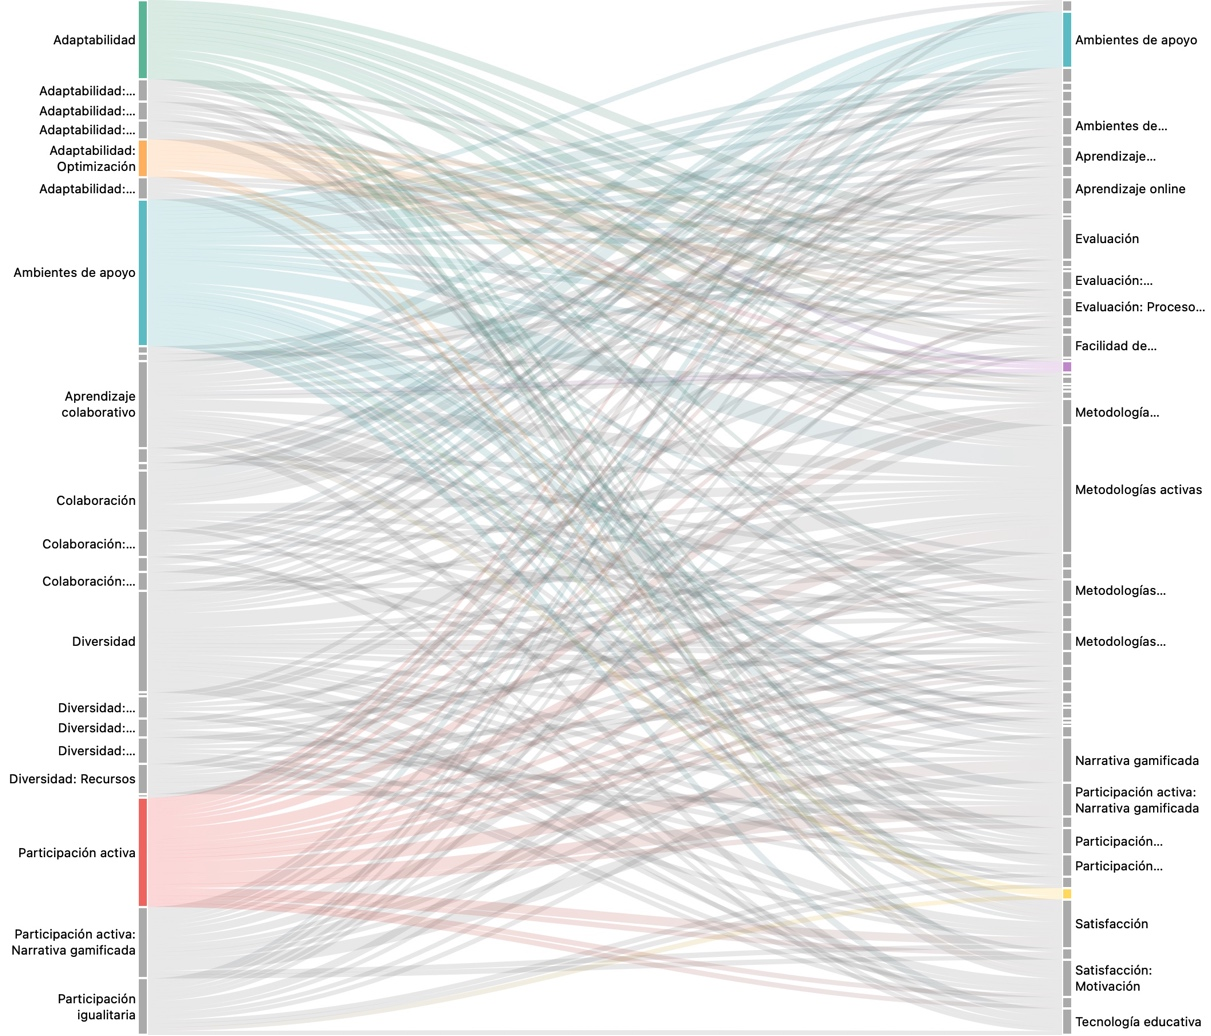
\includegraphics[width=\textwidth]{Imagem13.png}
\source{Elaboración propia.}
\end{minipage}
\end{figure}

\section{Conclusão}\label{sec-conclusao}

Buscamos investigar o potencial de um ambiente imersivo na aprendizagem de
vocabulário de inglês como LE, observando, em particular, sua capacidade de
promover atenção e motivação nos alunos. Para responder às perguntas de
pesquisa, foram realizados três experimentos com alunos de nível elementar de
proficiência em língua inglesa de um colégio de aplicação em Minas Gerais.

A partir dos resultados dos testes de vocabulário, verificou-se que houve ganho
de aprendizagem nas três condições de testagem, respondendo positivamente à
primeira pergunta de pesquisa: ``\emph{O ambiente imersivo em 360º contribui para a
aprendizagem de vocabulário de inglês como língua estrangeira?}''. Além disso,
verificou-se que o ambiente imersivo em 360º, ao proporcionar uma experiência
nova aos alunos através da imersão e da multimodalidade, é capaz de fazer com
que se sintam mais motivados e, assim, direcionem melhor sua atenção ao objeto
de aprendizagem \cite{gardner2010}, o que resulta em mais \emph{noticing} \cite{schmidit1990}
e possibilita o aprendizado do vocabulário, respondendo também afirmativamente
à segunda pergunta: ``\emph{O ambiente imersivo em 360º contribui para promoção da
motivação e da atenção durante o aprendizado do vocabulário de inglês como
LE?}''.

Ainda, verificou-se que o ganho de aprendizagem foi mais expressivo em uma
condição que em outras. Assim, calculou-se o ganho médio de aprendizagem
lexical para cada grupo. Os grupos expostos ao ambiente imersivo em 360º, ao
ambiente de leitura com glossário multimodal e ao ambiente imersivo em 360º +
ambiente de leitura com glossário multimodal apresentaram ganho médio de
aprendizagem de, respectivamente, 18\%, 28\% e 62\%. Logo, responde-se à terceira
pergunta de pesquisa (``\emph{Comparativamente, qual das três condições testadas –
ambiente imersivo em 360º, ambiente hipermodal de leitura com glossário ou
ambiente imersivo em 360º + ambiente hipermodal de leitura com glossário – é
mais eficiente para a aprendizagem de vocabulário em LE?}''), pois a condição
mais eficiente para a aprendizagem de vocabulário foi a terceira, com 62\%. Isso
evidencia a importância do verbal e da apresentação simultânea das diferentes
modalidades aos alunos de nível elementar \cite{procopio2016}, pois os grupos que
contaram com um suporte da escrita (grupos 2 e 3), simultaneamente às imagens,
obtiveram maior ganho de aprendizagem que o grupo que contava apenas com as
modalidades sonora e visual (grupo 1).

Conclui-se que o ambiente imersivo em 360º tem um grande potencial pedagógico,
pois, ao apresentar o estímulo de forma multimodal, contribui
significativamente para o aprendizado e a retenção do vocabulário da LE, como
mostra a literatura \cite{chun1996,saito2015,procopio2016,mayer2001,monteiro2021}.
Ademais, ele é uma alternativa mais acessível para a
inserção da RV em salas de aula de LE, pois é mais econômica e propicia a
interação do aprendiz com elementos virtuais de forma dinâmica, fazendo com que
ele engaje mais nas atividades propostas.

Contudo, algumas limitações precisam ser apontadas, como a impossibilidade de
reproduzir as pronúncias das palavras no glossário devido à falta de
dispositivos de reprodução de som nos computadores da escola, impedindo que os
alunos acessassem uma das modalidades presentes do ambiente (a sonora). Outra
limitação que precisa ser destacada é a impossibilidade de inserir um glossário
multimodal no ambiente imersivo em 360º, o que permitiria a consulta das
palavras alvo de forma simultânea à sua exploração, oferecendo um suporte
verbal durante a atividade.

Ainda, mais estudos precisam ser desenvolvidos para que o uso ambientes de RV
seja cada vez mais popularizado e integrado ao ensino de LE, estando cada vez
mais presente nas salas de aula brasileiras. Há também necessidade de modelos e
teorias de ASL que considerem em suas abordagens atenção e motivação de forma
integrada e como elementos centrais do processo de aprendizagem de línguas,
visto que esses construtos, quando abordados, o são de forma periférica e não
integrados em estudos encontrados na literatura \cite{krashen1985,ellis1997,gass1997,hede2002,mayer2002,moreno2007,saito2015,monteiro2021}.


\section*{Agradecimentos}\label{sec-agradecimento}

O primeiro autor agradece à Fundação Calouste Gulbenkian, no âmbito do
programa de apoio à formação dos PALOP e de Timor-Leste. Além disso, o
último autor agradece aos Fundos Portugueses, através da FCT Fundação
para a Ciência e a Tecnologia, no âmbito dos Projectos UIDB/00013/2020,
UIDP/00013/202.


\printbibliography\label{sec-bib}
%conceptualization,datacuration,formalanalysis,funding,investigation,methodology,projadm,resources,software,supervision,validation,visualization,writing,review
\begin{contributors}[sec-contributors]
\authorcontribution{Cacilda Helena Chivai}[conceptualization,funding,investigation,software,writing,review]
\authorcontribution{Armando Assunção Soares}[formalanalysis,resources]
\authorcontribution{Paula Catarino}[methodology,projadm]
\end{contributors}
\end{document}
